\section{Software Teori}
\textit{I dette afsnit beskrives den benyttede microcontroller, CY8CKIT-043 PSoC 4 M, og dennes egenskaber. Dette gøres med henblik på at opnå forståelse for dens muligheder, og hvordan disse kan benyttes til udvikling af systemet. \newline
Rapportens mikrokontroller enhed er udlånt af Aalborg Universitet og er af typen CY8CKIT-043 PSoC 4 M.}

\subsection{Mikrokontroller}
En mikrokontroller enhed (MCU) er et elektrisk system, som kan kontrollere elektronisk udstyr ved hjælp af indkorporeret softwaredesign. En MCU er dermed en mindre computer, der forefindes i elektroniske enheder. Eksempelvis er mikrokontrollere at finde i fjernsyn, mobiltelefoner og printere. \citep{Scienceuddannelse,Tanenbaum2006} \newline
Mikrokontrollere kan være bestående af en eller flere mikroprocessorer, hukommelse samt programmerbare in- og output-enheder. Dette giver brugeren af mikrokontrolleren mulighed for at programmere enheden således, at denne kan kontrollere henholdsvis in- eller output-enheder. \citep{Scienceuddannelse,Tanenbaum2006}

\subsection{CY8CKIT-043 PSoC 4-M}
Rapportens system vil gøre brug af den tilgængelige mikrokontroller CY8CKIT-043 Programmable System on Chip (PSoC) 4 M-Series Prototyping Kit og programmet PSoC Creator 3.3.\\
CY8CKIT-043 PSoC 4 M-Series Prototyping Kit er en mikrokontroller som indeholder tre mikroprocessorer: to Programmable System-on-Chips (PSoC) og en Programmable Radio-on-Chip (PRoC), hvilket ses på \figref{fig:PSoC}. Den første PSoC, LP5, på MCU sidder på KitProg boardet, som er den del af MCUen hvor USB er placeret. LP5 kan indeholde software, der kan indlæses på en computer ved hjælp af USB stikket. Den bruges til at programmere og debug softwaren på target boardet af MCUen, hvorfor denne del kan knækkes af resten af stikket og fungere selvstændigt. Dette kræver dog, at softwaren først er programmeret på den anden mikroprocessorer, som er PSoC 4200M. Denne mikroprocessor fungerer som hovedcomputeren. Denne kan eksempelvis kodes til en høj ydeevne af analog til digital konvertering (ADC) ved brug af sin 12-bits SAR ADC. \newline
På undersiden af mikrokontrolleren er der placeret en PRoC med Bluetooth Low Energy (BLE). Denne PRoC har ikke samme antal muligheder for afbenyttelse i forhold til PSoC 4200M, idet BLE er mere pladskrævende end PSoC 4200M. \citep{CYPRESS2016PSoC,Semiconductor2016,CYPRESS2016Cortexm0}
%
\begin{figure}[H]
	\centering
	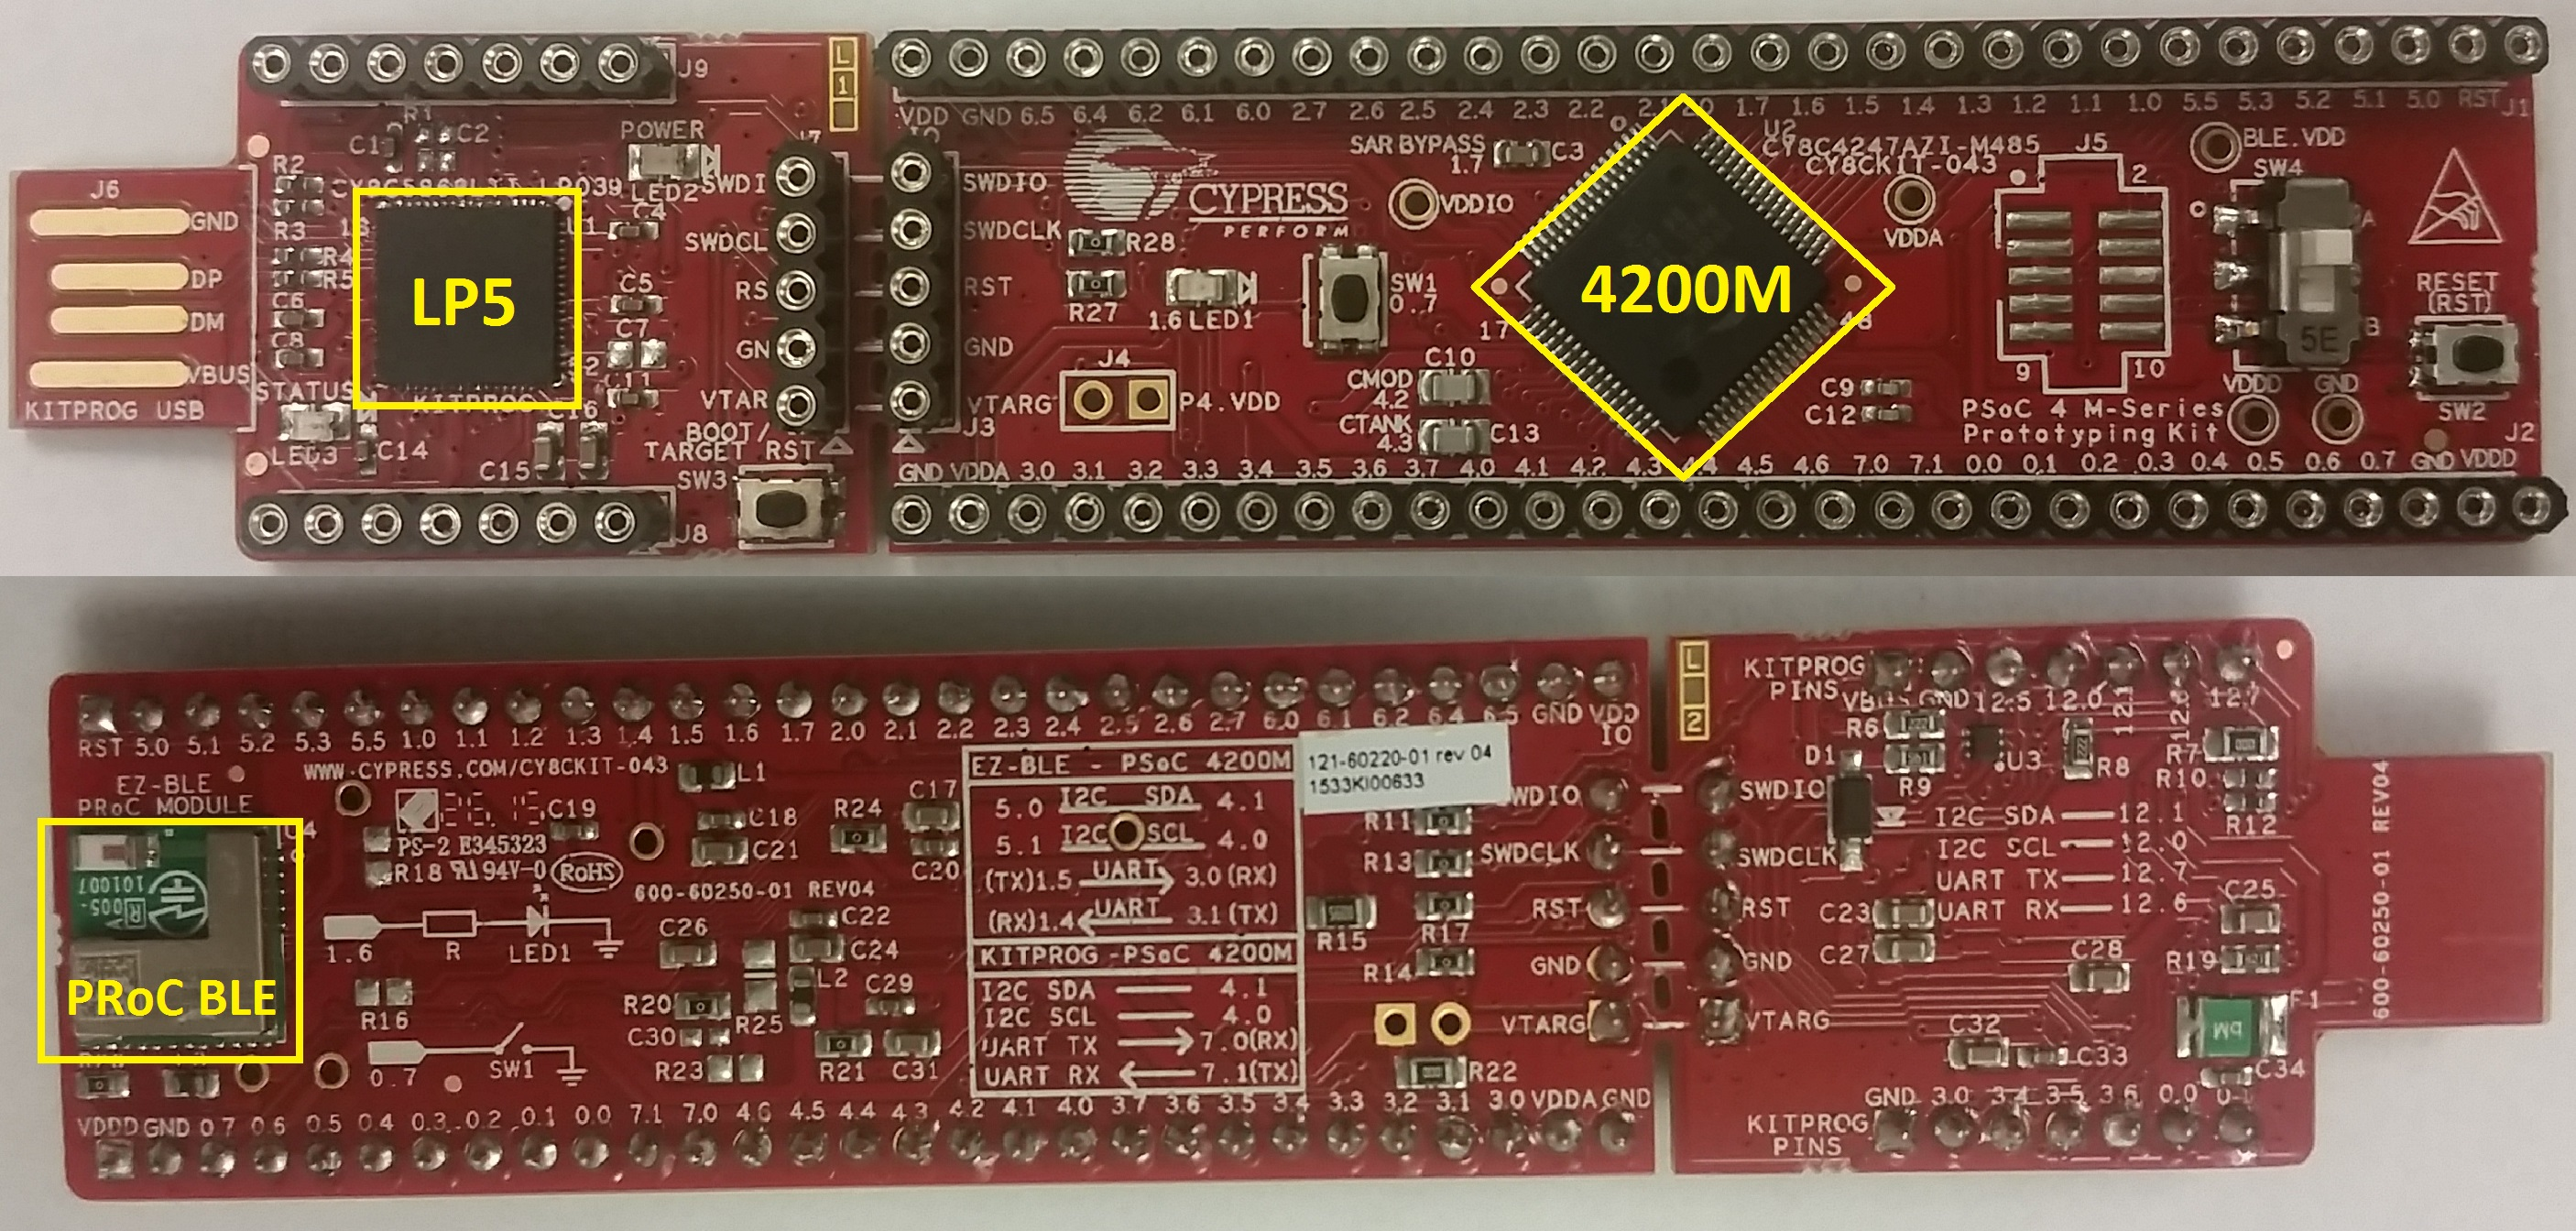
\includegraphics[scale=0.15]{figures/bProblemloesning/PSoC3.jpg}
	\caption{MCUen, CY8CKIT-043 PSoC 4 M-Series Prototyping Kit, er vist på forsiden og undersiden. MCUens PSoC, LP5 og 4200M, samt PRoC BLE er markeret med gul.\newline
	%Mikrokontrolleren kan knækkes over i to: KitProg board med USB stik og target board med hovedchippen PSoC 4200M\fxnote{Navnene er fundet nederst på side 26 i manualen}. PRoCen er ikke påmonteret som standard fra Cypress, hvorfor denne er blevet loddet manuelt på efterfølgende.
	 Kontakten helt til højre på forsiden af target boardet, skal trykkes ned for, at PRoC programmeres på istedet for PSoC 4200M. \citep{CYPRESS2016PSoC,Semiconductor2016}}
	\label{fig:PSoC}
\end{figure}\vspace{-0.2cm}
%
For at opsamle data benyttes to MCUer, hvoraf den ene fungerer som GAP central og den anden som GAP peripheral. GAP central er tilkoblet en ekstern enhed, såsom en computer, gennem USB samtidig med at GAP peripheral er placeret på det objekt som data skal opsamles fra. Dataoverførslen mellem disse to enheder, vil derfor foregå gennem brug af Bluetooth. I dette tilfælde benyttes en MCU fra Cypress, hvormed GAP central og GAP peripheral omtales som henholdsvis GAP central og GAP peripheral \citep{Luthra2015}. \newline

Kommunikationen mellem en master og en slave i et integreret system kan lade sig gøre ved brug af enten Serial Peripheral Interface (SPI) eller Inter-Integrated Circuit (I$^{2}$C) interface. Disse interface er kommunikationsprotokoller som benyttes internt i eksempelvis MCUer, til at kommunikation mellem mikroprocessorer. Mellem mikroprocessorerne forefindes dermed serielle porte med to ledninger til at sende data (TX) og modtage data (RX). \citep{Semiconductor2016} \newline
SPI er en kommunikationsprotokol som blandt andet benyttes til full-duplex kommunikation, hvilket giver mulighed for henholdsvis at sende og modtage data. En SPI bus involverer én master og et givent antal slaver. SPI busser benytter derfor 4 ledninger til at skabe forbindelser mellem disse enheder. I tilfælde af, at der er benyttes flere slaver til én master, da er det påkrævet at alle slaver har hver sin chip select. SPI er dog en hurtig kommunikationsprotokol, på trods af sine pladskrævende elementer ved et større antal slaver tilkoblet. \citep{Semiconductor2016,Sparkfun2016} \newline
Yderligere forefindes I$^{2}$C, som ligeledes er en computerbus dataprotokol. Masteren i systemet kontrollerer I$^{2}$C bussen og sender kommandoer til slaven. Både masteren og slaven kan sende og modtage data, men masteren kontrollerer, hvornår dette kan finde sted. \newline
I$^{2}$C kan, modsat SPI, involverer flere mastere til kommunikation med et givent antal slaver. Ydermere er I$^{2}$C en mere kompleks kommunikationsprotokol, men samtidig mindre pladskrævende end SPI. Dette skyldtes, at I$^{2}$C blot kræver 2 ledninger, hvor I$^{2}$C kræver 4 ledninger til at skabe forbindelse mellem master og slave. \citep{Semiconductor2016,Sparkfun2016}

En MCU kræver en ekstern strømkilde for at kunne fungere. Ved forbindelse med en USB port adapteres spændingsforsyningen til 5V, men det er yderligere muligt at tilkoble en spænding til MCUens lav-volt applikation, hvilket gør den trådløs. \newline
Den benyttede MCU påkræver en spændingstilkobling i området 1,71~V til 5,50~V, når MCUen ikke er tilkoblet en USB port. Dermed skal VDD tilsluttes dette spændingsinterval fra en reguleret spændingsforsyning, for at overholde MCUens arbejdsområde. \citep{Semiconductor2016,Semiconductor20164200M}

Programmet PSoC Creator kan designe hardware og software til MCUen. Dette program benyttes til at designe og kode MCUens, hvorved softwaren kan tilpasses de fysiske komponenter i C kodning. \citep{Semiconductor2016} \\
Når MCUen er tilsluttet computeren og debugger ved brug af PSoC creator, kan MATLAB fungere som et grafisk bruger interface (GUI). Dette muliggør realtime visualisering af den data, som eksempelvis en GAP central MCU modtager fra en GAP peripheral MCU.\citep{Semiconductor2016,Sparkfun2016}

\subsection{ADC}
En analog-til-digital konverter benyttes, når et analog signal skal konverteres til digital data, som kan bearbejdes eller visualiseres af en digital enhed. Samplingsfrekvensen og opløsningen for ADCen er afgørende for, hvor repræsentativt det analge signal bliver gengivet i den digitaliserede udgave. Ifølge Nyquists teori skal samplingsfrekvensen være mindst det dobbelte af den højeste frekvens i signalet, for at sikre en repræsentativ gengivelse af det analoge signal. Der findes flere forskellige typer ADC, som for eksempel digital ramp ADC, sigma delta ADC og successive approximation (SAR) ADC. En digital ramp ADC tæller op fra 0 V for at finde det rette niveau for inputspændingen fra signalet. Når den rammer signalets spænding, overføres denne værdi til et digitalt output, referencespændingen nulstilles og tæller forfra igen. En sigma delta ADC oversampler og besidder kun en 1 bits konverter. Den foretager en sammenligning af en reference værdi med inputspændingen, som enten giver 0 eller 1 som output. Alle disse værdier indsendes til et digitalt filter, der indsætter antallet af digitale ettaller og derved konverterer til et digitalt signal. Forskellen herimellem er altså metoden for konverteringen. \citep{Moore2004,Sheingold2014} \\
I mikrokontrolleren findes en 12 bits 1 mega sample per sekund (Msps) SAR ADC. I en SAR ADC kommer signalet ind i en komparator, der har en spændingsværdi og sammenligne med (Vref). Først sammenlignes inputsignalet med Vref, som indstilles til at være halvdelen af arbejdsområdet. Komparatoren vil vurdere, om signalet er større eller mindre end denne værdi. Herved findes det mest betydende tal, hvorefter processen med halvering af Vref, som lægges til eller trækkes fra, og vurdering herudfra fortsætter indtil de 12 bits er fundet. Derved er den analoge data konverteret til binære tal. Hvis en SAR ADC har for mange bits, bliver disse inddelingstrin så små, at det kan være støj, som afgør bits trinet. \citep{Moore2004,Sheingold2014} Et eksempel på en SAR ADC's virkemåde ses på \figref{fig:SAR_ADC}
\begin{figure}[H]
	\centering
	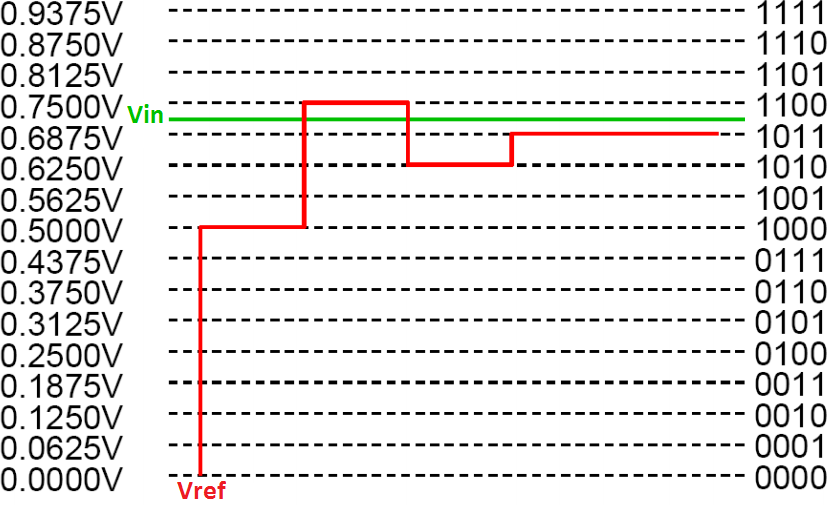
\includegraphics[scale=0.6]{figures/bProblemloesning/SAR_ADC.png}
	\caption{På figuren ses en 4 bits SAR ADC's virkemåde. Vin har i dette tilfælde en fast værdi, men kan skifte mange gange i sekundet. Om ADC'en kan opfange dette afhænger af samplingshastigheden og antallet af bits. Vref indstilles til halvdelen af arbejdsområdet på 1 V. Her vurderer komparatoren, at inputsignalet er større end Vref, hvorfor første betydende tal er 1. Derefter lægges en fjerdedel af arbejdsområdet til Vref og komparatoren vurderer igen. Dette fortsætter til alle fire bits er fundet, og det analoge signalet er derved konverteret til digitalt.}
	\label{fig:SAR_ADC}
\end{figure}\vspace{-0.5cm}
Mikrokontrollerens 12 bits ADC kan inddele det analoge signal i $2^{12} = 4096$ spændingsniveauer og skal bruge 18 clocks for at fuldføre en 12 bits konvertering af data med samplingsfrekvens på 18.000.000 Hz, hvilket er dens maksimale samplingsfrekvens. Den understøtter både single ended og differential inputs og kan skanne alle 16 kanaler automatisk. \citep{Semiconductor20164200M,Moore2004}

\subsection{Interrupts}
Interrupt er en funktion, som kan afbryde CPU'ens main fil ved at løfte et ben højt, hvis en bestemt hændelse sker eller en timer har talt op til et bestemt niveau. Dette kan være behjælpeligt for CPU'en, da den herved ikke skal tjekke konstant for, om en bestemt hændelse sker. \citep{Badiger2016} \\
I en aktivitetsmåler kan interrupts blandt andet benyttes til at aktivere gyroskopet til detektion af cykling. Hvis denne aktivitetsform ikke finder sted, lægges benet for funktionen ned igen og aktivitetsmåleren fortsætter som ellers.

En PSoC 4 besidder 32 interrupt linjer, IRQ[0] til og med IRQ[31], som kan prioriteres efter fire niveauer. %Derudover findes en Wakeup Interrupt Controller (WIC), som vækker processoren op fra deep sleep mode. 
Når et interrupt finder sted, vil CPU'en modtage en specifik funktion, som kaldes Interrupt Service Routine (ISR). Denne skal sørge for, at interruptets kode overståes hurtigst muligt, hvorved mainprogrammet ikke afbrydes konstant. Interruptets kode bliver eksekveret, hvorefter main filen fortsættes. \citep{Badiger2016}\\
Inden et interrupt er mainen i tread mode, hvilket ses på \figref{fig:interrupt}. Når interruptet finder sted, vil en pind gå høj, og processoren vil overføre information til den nuværende stack. Dette kaldes for stacking, hvilket får main filen til at gå i handler mode. Her skifter pointeren også stilling, hvorfor den går fra Main Stack Pointer (MSP) til Process Stack Pointer (PSP). Dette betyder, at den pågældende funktion gemmes og sættes på pause. Det er derved muligt at vende tilbage til præcis samme sted i processen efter interruptet. ISR kører sit program, hvorefter pinden lægges ned igen og unstacking foregår. Main filen går igen i tread mode, pointeren skifter til MSP og hovedarbejdet fortsættes. Alt dette ses på \figref{fig:interrupt}. \citep{Badiger2016,Tanenbaum2006}
\begin{figure}[H]
	\centering
	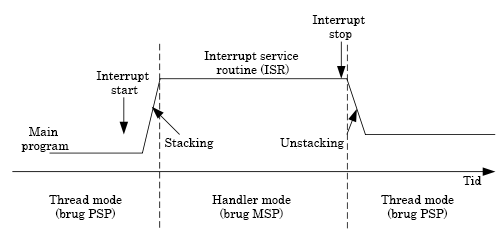
\includegraphics[scale=0.68]{figures/bProblemloesning/interrupt.png}
	\caption{På figuren ses et overblik over, hvad der sker når et interrupt afbryder CPU'ens main. \citep{Tanenbaum2006}}
	\label{fig:interrupt}
\end{figure}\vspace{-0.5cm}
I en ARM Cortex-M0 kan en høj prioritet afbryde en lav prioritet. Hver gang et interrupt finder sted, er der risiko for et stack overflow. Dette hænder, hvis afbrydelserne fortsætter i uendelighed, og det ikke er muligt af finde ud af, hvor i prosessen interruptet skal vende tilbage til. %Hver gang der sker et interrupt skal otte 32-bits word på stacken. 
Igennem unstacking genskabes de registre fra, hvor afbrydelsen oprindeligt fandt sted. \citep{Badiger2016}

Der findes forskellige slags interrupts, som blandt andet kan finde sted på grund af manuel udløsning eller algoritmer. Næsten alle interrupts er programmerbare i PSoC 4 udstyr. Der findes dog fem interrupts, som ikke kan ignoreres og kaldes exeptions. Disse er prioriteret højere end alle andre interrupts, da de beskytter og sikre mod fejl. \fxnote{Watch Dog timeren genstarter og har aller højest prioritet af alle interrupts}\citep{Badiger2016}
% Der findes to typer kilder til PSoC 4 interrupts: Fixed-function interrupt sources eller Universal Digital Block (UDB). Fixed-function interrupts er definerede interruptskilder fra on-chip perifert udstyr, som kan udløse manuelt. Herimod kan ethvert digitalt signal, som er genereret i en UDB, udløse et interrupt. Disse to typer er begge programmerbare eksterne interrupts, som i ARM Cortex M0 mikroprocessoren har lavest prioritet. Der findes fem yderligere interrupts, som kaldes exeptions og er prioriteret højere end de programmerbare eksterne interrupts. Disse eksisterer for blandt andet at genstarte processoren i tilfælde af softwarefejl\fxnote{Watch Dog timeren genstarter og har aller højest prioritet af alle interrupts}. \citep{Badiger2016}

\subsection{Clocks}
Clocks er et kredsløb, som benyttes til at synkronisere for eksempel rækkefølgen af funktioner eller indstilling af to signaler. Det kan siges, at en clock kontrollerer tiden for et program. En clock udsender ved hjælp af oscillatorer en række impulser, der skifter mellem værdierne 0 og 1 og har præcis pulsbredde og interval mellem hinanden. Tidsintervallet imellem henholdsvis to pulsers stigning fra 0 til 1 eller fald fra 1 til 0 %to impulsers stigning til 1 eller fald fra 1 
kaldes clock cycle time, og pulsfrekvensen indstilles herefter. Pulsfrekvensen styres ofte kontrolleret af en crystal oscillator, da dette gør frekvensen mere præcis. \citep{Tanenbaum2006}

En clock er et helt grundlæggende element i mikrokontrollere. Den kan eksempelvis bruges til at lave interrupts på bestemte tidspunkter, hvis der er behov for, at en funktion skal køres igennem på bestemte tidspunkter\xnote{Når gyroskopet skal vækkes op hvert tiende skund}. Derudover kan en clock for eksempel benyttes som måleenhed for funktioners varighed. Derved opnås bevidsthed om, hvornår to funktioner skal påbegyndes, hvis de har forskellige clock cykles men skal være afsluttet samtidig. \citep{Tanenbaum2006}

Clock systemet for PSoC 4200M består af en Watch Crystal Oscillator (WCO), der kører med 32 kHz. Derudover findes en internal main oscillator (IMO), som kører med 24 MHz men kan fungere fra 3 til 48 MHz, og en internal low-speed oscillator (ILO), der nominalt kører med 32 KHz. IMO er den primære kilde til intern clocking indeni PSoC 4200M i aktiv tilstand, hvorimod ILO kan generere clocks under deep sleep mode. WCO kan både benyttes under aktiv og deep sleep mode. Denne oscillator kan desuden benyttes som en real-time clock, hvilket holder styr på den aktuelle tid.\fxnote{Når vi ved, om vi skal bruge clocks, og i så fald hvilke, kan disse eventuelt blive beskrevet her.} \citep{Semiconductor20164200M}
%http://www.hardwaresecrets.com/how-a-cpu-works/2/

\subsection{Mikrokontrollerens target CPU}
Mikroprocessoren, 4200M, er target CPU'en på CY8CKIT-043 PSoC 4 M-Series Prototyping Kit. Denne mikroprocessor indeholder den kodning som foretages i PSoC Creator, og er dermed indeholdende de instruktionerne som skal eksekveres når systemet er funktionelt. Mikroprocessoren, 4200M, besidder ydermere en ARM cortex-M0 processer. \newline
Mikroprocessoren er basseret på Instruction Set Architecture (ISA). ISA er bindeleddet mellem MCUens hardware og software, hvormed C kodningen af softwaren muliggør at instruktioner kan blive udført i forbindelse med MCUens hardware. ISA's kategorier kan blandt andet være Reduced Instruction Set Computer (RISC) eller Complex Instrucion Set Computer (CISC). \citep{CYPRESS2016Cortexm0,Semiconductor20164200M,Yadav2016} \newline
Den benyttede MCUs mikroprocessor, 4200M, er af kategorien RISC. RISC processorer benytter simple instruktioner, som kan blive eksekveret under én clock cycle. Derimod kræver dette mere RAM kapacitet, fordi hver opgave hentes ned, processeres over flere omgange og gemmes indtil de er eksekveret. Denne metode tillader dog pipelinning, hvilket gør at flere instruktioner kan køre samtidig. En CISC baseret computer vil derimod udføre opgaver med så få linjer som muligt. Processorens hardware vil dermed være opbygget til at forstå og udføre komplekse instruktioner, hvilket kræver flere transistorer end RISC metoden. \fxnote{fetch - decode - exicute. Mere laves samtidig} Sammenlignet er RISC processen hurtigere end CISC, men CISC computere kan udføre flere komplekse instruktioner på færre linjer end RISC. \citep{CYPRESS2016Cortexm0,Semiconductor20164200M,Yadav2016}\\
CPU'en i Cortex-M0 er en del af det 32-bit MCU delsystem, som optimerer energibesparende drift ved hjælp af clock gating\fxnote{Clock gating saves power by adding more logic to a circuit to prune the clock tree. Pruning the clock disables portions of the circuitry so that the flip-flops in them do not have to switch states. Switching states consumes power. When not being switched, the switching power consumption goes to zero, and only leakage currents are incurred}. %% Noget om deep sleep / low power mode (Hvis den har det), hvor mange registre den har og hvis nogen af dem har dedikerede funktioner
CPU'en har en flash hukommelse på 128 kB og en 16 kB RAM af typen SRAM. Algoritmen og dermed programmet for MCUen gemmes i flash hukommelsen, da RAM hukommelsen kræver konstant strøm og slettes dermed, hvis strømtilførslen til MCUen slukkes. \citep{Semiconductor20164200M}
%tilgængelige pins - tilkobling af perifære moduler, som f.eks. en sensor
%
\subsection{Trådløs kommunikation via Bluetooth Low Energy} 
Klassisk Bluetooth er fordelagtigt at benytte, hvis der ønskes trådlås kommunikation eller trådløse enheder. PRoC'ens CPU på CY8CKIT-043 PSoC 4 M-Series Prototyping Kit er EZ\_BLE PRoC Module, som besidder en ARM cortex-M0 processer.% og har produktnavnet CYBLE-022001-00. 
Denne CPU har en 2,4 GHz BLE radio, som understøtter en datahastighed på 1 Mbps, med en chip antenne, der kan transmittere data ved radiofrekvens mellem 2,4-2,5 GHz. %Rundt om antennen, som sender og modtager data, er der fri plads, fordi den larmer meget og vil dermed ødelægge radioens funktion samt data.
\citep{Semiconductor2016PRoC,Semiconductor2016BLEdyb}\\
Bluetooth er en radiobølge teknologi, som hovedsageligt er designet til trådløs kommunikation imellem enheder. Der findes Bluetooth Smart enheder, som kun understøtter BLE, og Bluetooth Smart Ready enheder, der understøtter både klassisk Bluetooth og BLE. Radiobølgerne bliver sendt og modtaget i bånd af 79 forskellige frekvenser, som kaldes kanaler. Bølgerne bliver modificeret af enheden, således de opfattes som et signal. Når to enheder forbindes med hinanden, danner de et netværk kaldet en piconet. Enheden, som skaber forbindelsen, vil automatisk være masteren og kan for eksempel kontrollere afsendelsen af data fra slaven samt styre varigheden af forbindelsen. Tilsammen vælger masteren og slaven en tilfældig kanal, men for at mindske risikoen for interferens fra andre enheder skifter de to kanal op til tusinde gange i sekundet. \citep{CYPRESS2016workshopBLE,Sauter2011} \\
BLE er en videreudvikling og kaldes også Bluetooth version 4.0. BLE kræver mindre strøm for at fungere, fordi enheden er i sleep mode størstedelen af tiden. Når data skal sendes, vil den aktivere og overføre så hurtigt som muligt for igen at deaktivere og gå i sleep mode. Dette opnås ved, at BLE kun benytter 40 forskellige kanaler, hvor nogle for eksempel er specielt dedikeret til at skabe forbindelse\fxnote{3 kanaler - klassisk bluetooth har 32} mellem enheder, og andre kanaler dedikeres til at sende data. Derved sikres en driftscyklus\fxnote{ratio mellem enheden er slukket og tændt} som er tæt på nul. Et BLE modul kan dog ikke skifte undervejs mellem master og slave rollen, hvilket betyder, at når en forbindelse er skabt, vil der være en fast master og en fast slave. Dette simplificerer designet yderligere, hvorved der ligeledes spares strøm. \citep{Gupta2013}